\chapter{电路文档}\label{sec8}

在前面章节中介绍电路的目的是帮助读者理解电路原理,所以有些电路仅给出了最简单的例子。在本章中,会直接给出一些电路的结果供参考。对于较难的电路会给出思路。

\section{传感器}
\begin{figure}[!ht]
    \centering
    
\includegraphics{images/221.png}
    \caption{区域重生感应器。在玩家进入世界或玩家复活后,首次进入傀儡附近时激活,有小延迟。}
\end{figure}
\begin{figure}[!ht]
    \centering
    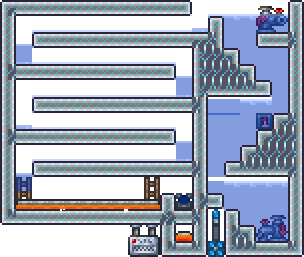
\includegraphics[width=0.45\textwidth]{images/11.png}
    \qquad
    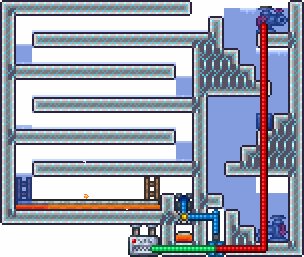
\includegraphics[width=0.45\textwidth]{images/12.png}
    \caption{开服感应器。在玩家进入世界时激活。}
\end{figure}
\begin{figure}[!ht]
    \centering
    
\includegraphics{images/309.png}
    \qquad
    
\includegraphics{images/310.png}
    \caption{血月感应器。打开一秒计时器后,压力板会不断激活。}
\end{figure}
\begin{figure}[!ht]
    \centering
    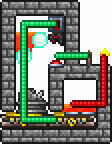
\includegraphics{images/311.png}
    \caption{血月\&雨天感应器。打开一秒计时器后,血月时右边火把不断激活,雨天且不是血月时左边火把不断激活。}
\end{figure}
\begin{figure}[!ht]
    \centering
    
\includegraphics{images/312.png}
    \caption{击退感应器。玩家被击退时传送走。用于检测穿墙怪。}
\end{figure}

\section{递次电路}
\subsection{传统递次电路}\label{sec2}
\mbox{}
\begin{figure}[!ht]
    \centering
    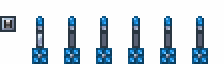
\includegraphics{images/72.png}
    \qquad
    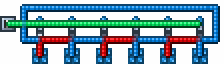
\includegraphics{images/73.png}
    \caption{传统递次}
\end{figure}
\begin{figure}[!ht]
    \centering
    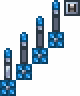
\includegraphics{images/78.png}
    \qquad
    
\includegraphics{images/79.png}
    \caption{斜式传统递次}
\end{figure}
\begin{figure}[!ht]
    \centering
    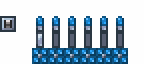
\includegraphics{images/82.png}
    \qquad
    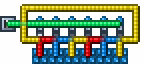
\includegraphics{images/83.png}
    \caption{密排传统递次}
\end{figure}
\begin{figure}[!ht]
    \centering
    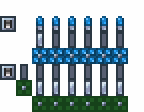
\includegraphics{images/317.png}
    \qquad
    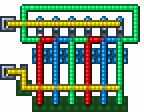
\includegraphics{images/318.png}
    \caption{密排带复位传统递次}
\end{figure}
\begin{figure}[!ht]
    \centering
    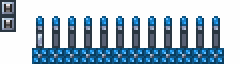
\includegraphics{images/106.png}
    \qquad
    
\includegraphics{images/107.png}
    \caption{带复位的传统递次}
\end{figure}

\subsection{传统双向递次电路}\label{sec3}
\mbox{}
\begin{figure}[!ht]
    \centering
    
\includegraphics{images/263.png}
    \qquad
    
\includegraphics{images/264.png}
    \caption{传统双向递次}
\end{figure}
\begin{figure}[!ht]
    \centering
    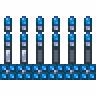
\includegraphics{images/261.png}
    \qquad
    
\includegraphics{images/262.png}
    \caption{密排传统双向递次}
\end{figure}

\begin{figure}[!ht]
    \centering
    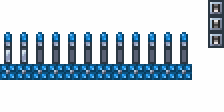
\includegraphics{images/265.png}
    \qquad
    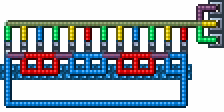
\includegraphics{images/266.png}
    \caption{带复位的传统双向递次}
\end{figure}

\subsection{多级递次电路}\label{sec5}
\mbox{}
\begin{figure}[!ht]
    \centering
    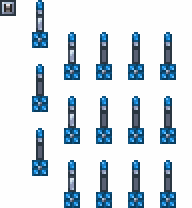
\includegraphics{images/313.png}
    \qquad
    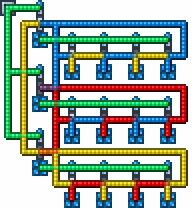
\includegraphics{images/314.png}
    \caption{周期为12的二级递次}
\end{figure}
\begin{figure}[!ht]
    \centering
    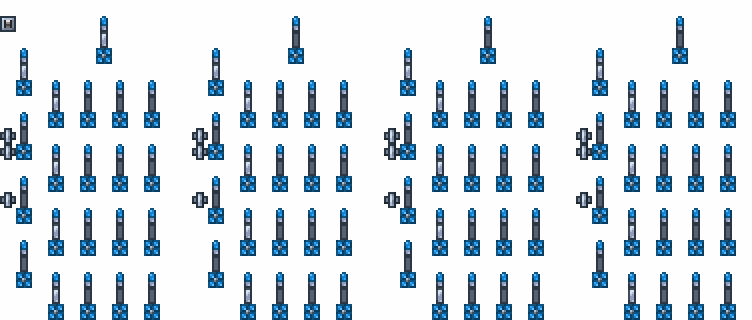
\includegraphics[width=\textwidth]{images/316.png}
    
    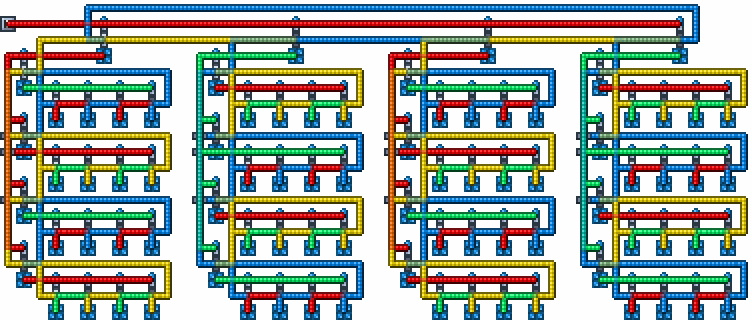
\includegraphics[width=\textwidth]{images/315.png}
    \caption{周期为64的三级递次}
\end{figure}

\subsection{推广递次电路}
\mbox{}
\begin{figure}[!ht]
    \centering
    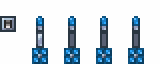
\includegraphics{images/84.png}
    \qquad
    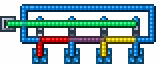
\includegraphics{images/85.png}
    \caption{周期为15的推广递次}
\end{figure}
\begin{figure}[!ht]
    \centering
    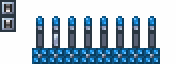
\includegraphics{images/319.png}
    \qquad
    
\includegraphics{images/320.png}
    \caption{带复位的推广递次}
\end{figure}

\section{降频电路}
\subsection{固定数值的降频}
\begin{figure}[!ht]
    \centering
    
\includegraphics{images/327.png}
    \qquad
    
\includegraphics{images/328.png}
    \caption{降频2}
\end{figure}
\begin{figure}[!ht]
    \centering
    
\includegraphics{images/331.png}
    \qquad
    
\includegraphics{images/332.png}
    \caption{降频3}
\end{figure}
\begin{figure}[!ht]
    \centering
    
\includegraphics{images/334.png}
    \qquad
    
\includegraphics{images/333.png}
    \caption{降频4}
\end{figure}
\subsection{交错数值的降频}
\begin{figure}[!ht]
    \centering
    
\includegraphics{images/330.png}
    \qquad
    
\includegraphics{images/329.png}
    \caption{降频1-2}
\end{figure}
\subsection{可变数值的降频}

\section{数字显示}
\subsection{BCD数显}
\subsection{十进制计数器}
\subsection{六进制计数器}
\begin{figure}[!ht]
    \centering
    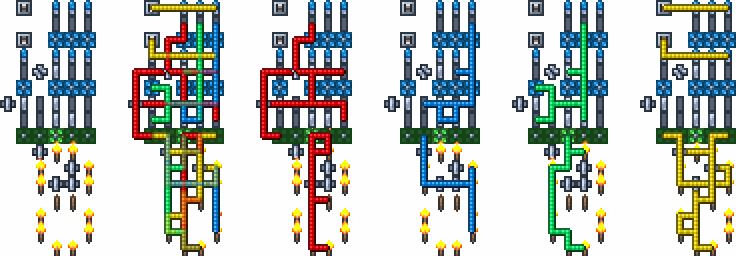
\includegraphics[width=\textwidth]{images/347.png}
    \caption{带复位六进制计数器}
\end{figure}
\subsection{月相显示}

\section{随机电路}
\subsection{随机多选一}
\subsection{随机分两组}
\begin{figure}[!ht]
    \centering
    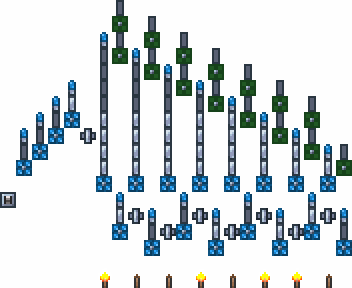
\includegraphics[width=0.45\textwidth]{images/134.png}
    \qquad
    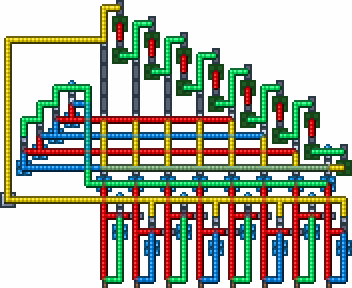
\includegraphics[width=0.45\textwidth]{images/135.png}
    \caption{随机八选四}
\end{figure}
\subsection{随机分多组}
\begin{figure}[!ht]
    \centering
    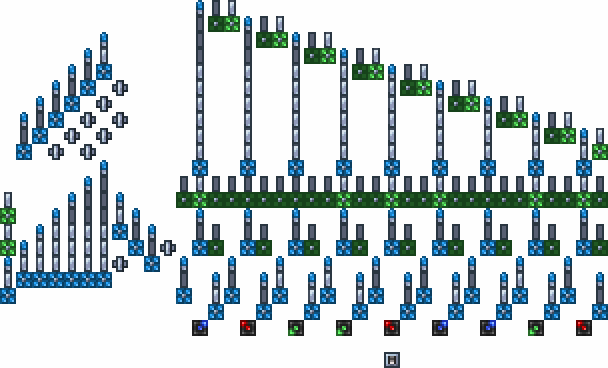
\includegraphics[width=0.45\textwidth]{images/148.png}
    \qquad
    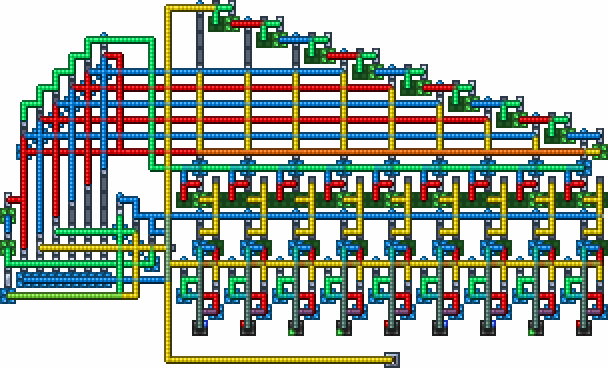
\includegraphics[width=0.45\textwidth]{images/149.png}
    \caption{九个输出随机分成3+3+3,占地最小}
\end{figure}
\begin{figure}[!ht]
    \centering
    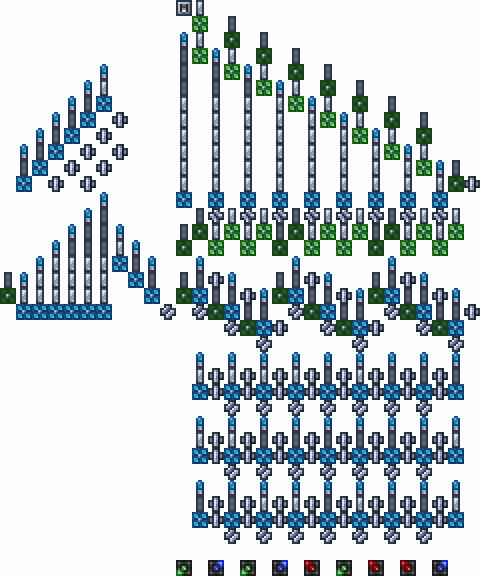
\includegraphics[width=0.45\textwidth]{images/146.png}
    \qquad
    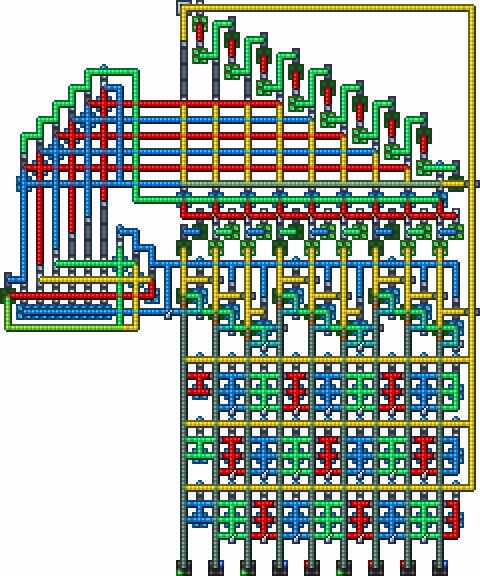
\includegraphics[width=0.45\textwidth]{images/147.png}
    \caption{九个输出随机分成3+3+3,最窄}
\end{figure}

\section{操纵板}
高频三向操纵板

\begin{figure}[!ht]
    \centering
    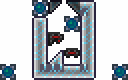
\includegraphics{images/253.png}
    \qquad
    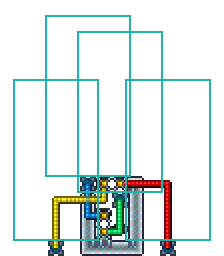
\includegraphics{images/254.png}
    \caption{低频四向操纵板(设计1)}
\end{figure}
低频四向操纵板

\section{像素盒显示器}

\section{矩阵显示器}

\section{算术电路}
\subsection{加减乘除}
\subsection{状态位运算}
\subsection{激活位运算}
\subsection{移位}

\section{存储器}
RAM设计123
\begin{figure}[!ht]
    \centering
    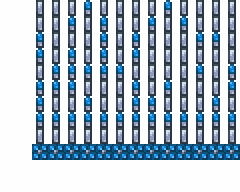
\includegraphics{images/342.png}
    \qquad
    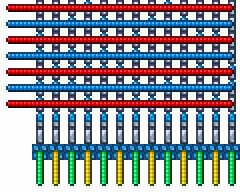
\includegraphics{images/341.png}
    \caption{ROM设计1,横向输入纵向输出}
\end{figure}
\begin{figure}[!ht]
    \centering
    \includegraphics{images/343.png}
    \qquad
    \includegraphics{images/344.png}
    \caption{ROM设计2,纵向输入横向输出}
\end{figure}
\begin{figure}[!ht]
    \centering
    \includegraphics{images/346.png}
    \qquad
    \includegraphics{images/345.png}
    \caption{ROM设计3,纵向输入横向输出}
\end{figure}
栈